\section{Auswertung}
Der genutze Laser hat eine Wellenlänge von \SI{623.99}{\nano\meter}.

\subsection{Kontrast des Interferometers}
Um den maximalen Kontrast des Interferometers zu bestimmen, wird für jeden Polarisationswinkel $\phi$  der Kontrast aus den Diodenspannungen der Intensitätsmessung mit Formel \ref{eqn:Kontast} berechnet und in Tabelle \ref{tab:Kontrast} aufgelistet.
Weiterhin werden in Abbildung \ref{fig:Kontrast} die berechneten Kontraste gegen den Polarisationswinkel aufgetragen und eine Ausgleichsrechnung der Form

\begin{equation*}
  K = A \cdot |\sin(2 \phi)|
\end{equation*}

durchgeführt. Als maximaler Kontrast folgt
\begin{equation}
  K_\text{max} = A = \num{0.71(5)} \, .
  \label{eqn:Kontrast}
\end{equation}

Es ist deutlich zu sehen, dass der maximale Kontrast deutlich kleiner als eins ist.

\begin{figure}[H]
  \centering
  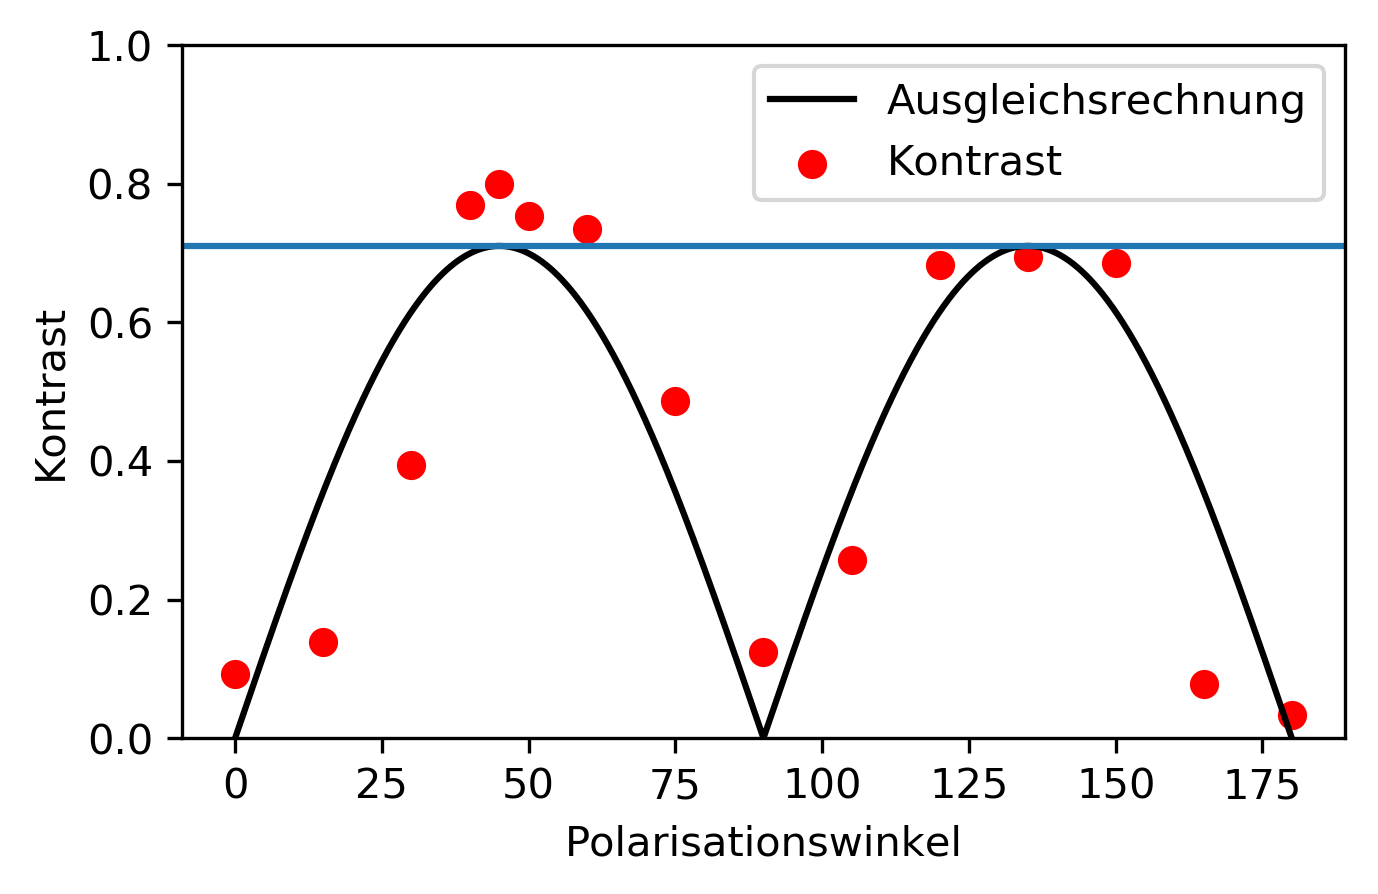
\includegraphics[width = .5\textwidth]{Auswertung/Plots/Kontrast.png}
  \caption{Kontrast des Interferometers in Abhängigkeit des Polarisationswinkels. }
  \label{fig:Kontrast}
\end{figure}

\begin{table}[H]
  \centering
  \caption{Spannungen $U_\text{min}$, $U_\text{max}$ und Kontrast $K$ des Interferometers in Abhängigkeit des Polarisationswinkels $\phi$.}
  \label{tab:Kontrast}
  \begin{tabular}{cccc}
    \toprule
    $\phi \, / \,  \si{\degree}$ & $U_\text{max} \, / \, \si{\volt}$ &  $U_\text{min} \, / \, \si{\volt}$ & Kontast \\
    \midrule
    0   & \num{1.060} &  \num{0.880} & \num{0.09} \\
    15  & \num{0.634} &  \num{0.479} & \num{0.14} \\
    30  & \num{0.560} &  \num{0.243} & \num{0.24} \\
    40  & \num{0.692} &  \num{0.090} & \num{0.76} \\
    45  & \num{0.855} &  \num{0.095} & \num{0.80} \\
    50  & \num{0.967} &  \num{0.136} & \num{0.70} \\
    60  & \num{0.972} &  \num{0.149} & \num{0.73} \\
    75  & \num{1.177} &  \num{0.406} & \num{0.49} \\
    90  & \num{1.216} &  \num{0.948} & \num{0.12} \\
    105 & \num{1.486} &  \num{0.878} & \num{0.26} \\
    120 & \num{2.550} &  \num{0.480} & \num{0.68} \\
    135 & \num{2.500} &  \num{0.450} & \num{0.70} \\
    150 & \num{2.580} &  \num{0.480} & \num{0.69} \\
    165 & \num{1.930} &  \num{1.650} & \num{0.08} \\
    180 & \num{1.100} &  \num{1.030} & \num{0.03} \\
    \bottomrule
  \end{tabular}
\end{table}


\subsection{Brechungsindex von Glas}

Zur Bestimmung des Brechungsindex von Glas werden die beiden Glasscheiben von \SI{-2}{\degree} bis \SI{9}{\degree} um die Ruhelage gedreht und die Anzahl Nulldurchgänge des Spannungssignals gezählt. Aus der Anzahl der Nulldurchgänge wird daraufhin anhand Gleichung \eqref{eqn:Brechungsindex} der Brechungsindex bestimmt. Dies wird zehn mal wiederholt. Für den Winkel der beiden Glasplättchen $\Theta$, den Rotationswinkel $\delta$, die Dicke $T$ der Glasplättchen sowie die Wellenlänge $\lambda_\text{HeNe}$ gilt

\begin{align*}
  \Theta &= \SI{10}{\degree} & \delta &= \SI{11}{\degree} \\
  T &= \SI{1}{\milli\meter}  & \lambda_\text{HeNe} &= \SI{623.99}{\nano\meter}
\end{align*}

In Tabelle \ref{tab:Glas} sind die Anzahl der Nulldurchgänge, sowie die daraus bestimmten Brechungsindeces aufgetragen. Für den Mittelwert des Brechungsindex von Glas folgt
\begin{equation}
  \overline{n} = \SI{1.54(2)} \, .
  \label{res:n_Glas}
\end{equation}

\begin{table}[H]
  \centering
  \caption{Anzahl der Nulldurchgänge und daraus berechnete Brechungsindeces der Glasplättchen.}
  \label{tab:Glas}
  \begin{tabular}{cc}
    \toprule
    \# Nulldurchgänge & Brechungsindex $n$ \\
    \midrule
    42 & \num{1.66} \\
    38 & \num{1.56} \\
    35 & \num{1.49} \\
    35 & \num{1.49} \\
    38 & \num{1.56} \\
    35 & \num{1.49} \\
    36 & \num{1.52} \\
    37 & \num{1.54} \\
    37 & \num{1.54} \\
    36 & \num{1.52} \\
    \bottomrule
  \end{tabular}
\end{table}

\subsection{Brechungsindex Druckzelle}

Zur Bestimmung des Brechungsindex von Luft in Abhängigkeit des Drucks werden in Abbildung \ref{fig:Druck_M} die gezählten Nulldurchgänge $M$ jeder Messung gegen den Druck $p$ aufgetragen. Aufgrund von Problemen bei der Versuchsdurchführung fehlen in den Messreihen einzelne Messwerte. Für jede Messreihe wird aus den Nulldurchgängen $M$ nach Formel \ref{eqn:Nulldurchgänge}
\begin{equation}
   n = \frac{\lambda}{L} M + 1
   \label{eqn:Nulldurchgänge}
\end{equation}
der Brechungsindex $n$ bestimmt und ebenfalls gegen den Druck in Abbildung \ref{fig:Druck_n} dargestellt. Für jede Messreihe wird außerdem eine lineare Ausgleichsrechnung der Form
\begin{equation}
  n(p) = m \cdot p + n_0
  \label{eqn:Fit}
\end{equation}
durchgeführt, die Parameter $m$ und $n_0$ dieser Ausgleichsrechnung sind in Tabelle \ref{tab:Druck} aufgelistet.
Weiterhin gilt nach dem Lorentz-Lorenz Gesetz für die Steigung $m$ der Funktion
\begin{equation*}
  m = \frac{3 A}{2 R T}
\end{equation*}
mit der Allgemeinen Gaskonstanten $R$, der molaren Refraktivität $A$ und der Temperatur $T$.
Um einen vergleichbaren Wert unter Normalbedingungen ($T_0 = \SI{15}{\degreeCelsius}$, $p=\SI{1}{\atm}$) zu erhalten, wird anhand der Parameter und Gleichung \eqref{eqn:Fit} der Brechungsindex bei für $p=\SI{1}{\atm}$ bestimmt und mit
\begin{equation*}
  m = m \cdot \frac{T}{T_0}
\end{equation*}
die Steigung angepasst. Die Raumtemperatur $T$ wurde am Ende der Messung an mehreren Stellen im Interferometer gemessen und der Mittelwert $T = \SI{295.3(7)}{\kelvin}\, \widehat{=}\, \SI{22.1(7)}{\degreeCelsius}$ bestimmt.

Die so berechneten Brechungsindices unter Normalbedingung sind in Tabelle \ref{tab:Druck} aufgetragen.
Für den Mittelwert dieser folgt
\begin{equation}
  \overline{n} = \SI{1.000275(2)}{} \,.
  \label{eqn:n_exp}
\end{equation}


\begin{table}[H]
  \centering
  \caption{Parameter der Ausgleichsrechnungen und die daraus relsultierenden Brechungsindices bei Normalbedingung. Die Steigung $m$ ist noch nicht, wie durch Gleichung \eqref{eqn:Fit} beschrieben, angepasst.}
  \label{tab:Druck}
  \begin{tabular}{ccc}
    \toprule
      Steigung $m$ & Achsenabschnit $n_0$ & Brechungsindex \\
      \midrule
      \SI{2.70(3)e-07}{} & \SI{1.000003(1)}{} & \SI{1.000283(3)}{} \\
      \SI{2.35(3)e-07}{} & \SI{1.000002(2)}{} & \SI{1.000246(3)}{} \\
      \SI{2.67(2)e-07}{} & \SI{1.000002(1)}{} & \SI{1.000279(2)}{} \\
      \SI{2.76(3)e-07}{} & \SI{1.000002(1)}{} & \SI{1.000288(3)}{} \\
      \bottomrule
  \end{tabular}
\end{table}

\begin{figure}[H]
  \centering
  \begin{subfigure}[l]{.49\textwidth}
    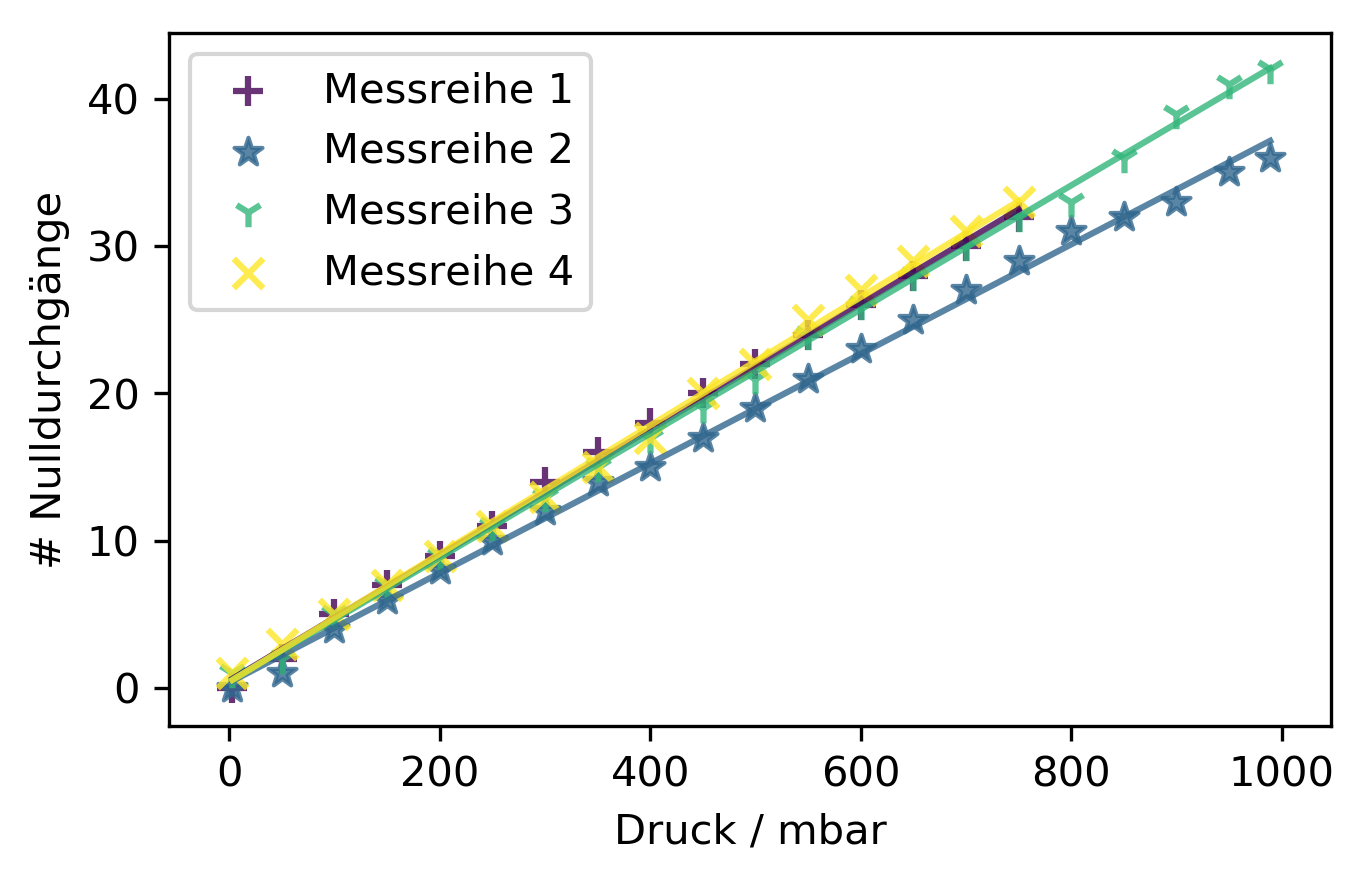
\includegraphics[width = \textwidth]{Auswertung/Plots/Messwerte.png}
    \label{fig:Druck_M}
  \end{subfigure}
  \begin{subfigure}[r]{.49\textwidth}
    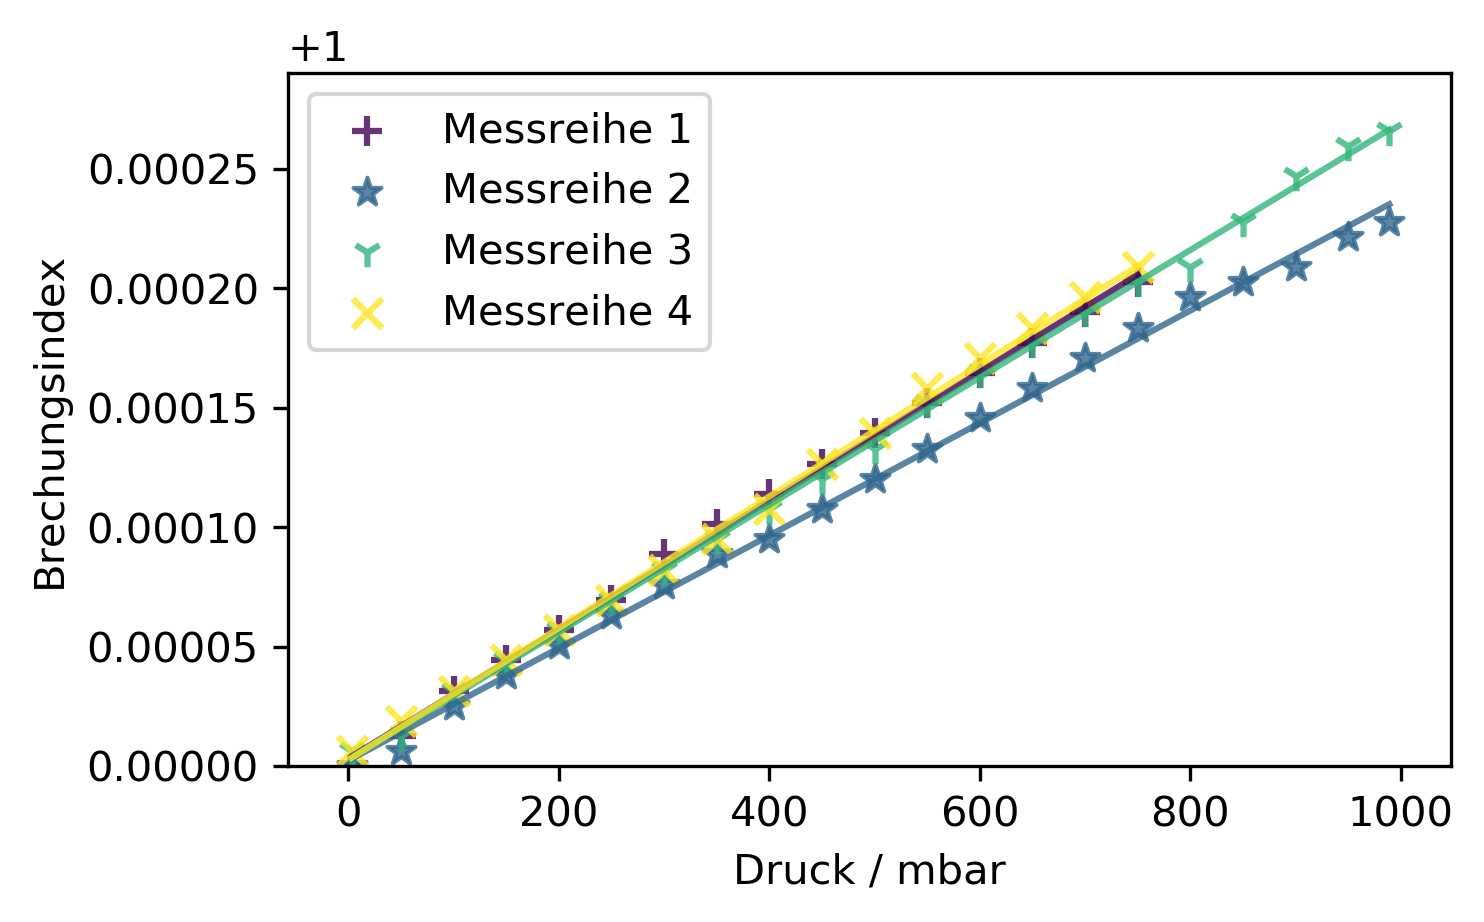
\includegraphics[width = \textwidth]{Auswertung/Plots/Brechungsindex.png}
    \label{fig:Druck_n}
  \end{subfigure}
  \caption{Brechungsindex von Luft als Funktion des Luftdrucks für vier Messreihen. Für die Messreihen 1. und 4. konnten für höhere Drücke keine Nulldurchgänge und somit auch kein Brechungsindex bestimmt werden.}
  \label{}
\end{figure}
